\documentclass[11pt,a4paper]{article}
\usepackage[T1]{fontenc}
\usepackage[utf8]{inputenc}
\usepackage[margin=22mm]{geometry}
\usepackage{amsmath,booktabs,graphicx,hyperref}
\title{Presupuesto de área para un píxel de NAUSICA}
\author{Registro de cálculo}\date{\today}
\begin{document}\maketitle
El pitch de 2 mm corresponde a una celda cuadrada de 4 mm$^2$.
Se estudia un presupuesto más exigente de 1 mm$^2$, con el pad de
0,5 mm de lado centrado y toda la electrónica situada fuera de su zona de
separación. Se adopta la arquitectura prevista en el manuscrito: lectura
multiplexada y ADC compartidos fuera del píxel. Los bloques locales de lectura
y control todavía se representan por reservas de área.

\section*{CSA calculado a partir del circuito}
Las dimensiones se leen directamente del netlist M3 x4, M4 x4. Se incluyen
las tres ramas paralelas de M2. M5 utiliza los parámetros efectivos de su
línea del netlist. La suma de áreas de canal es 706.647 $\mu$m$^2$.
\begin{center}\begin{tabular}{lrr}\toprule
Dispositivo & $W$ ($\mu$m) & $L$ ($\mu$m)\\\midrule
M1 & 220 & 0.5 \\
M2\_1 & 27 & 0.5 \\
M2\_2 & 27 & 0.5 \\
M2\_3 & 27 & 0.5 \\
M3 & 200 & 2 \\
M4 & 2.88 & 1.44 \\
M5 & 220 & 0.5 \\
M6 & 1 & 6 \\
Mf & 0.36 & 100 \\
\bottomrule\end{tabular}\end{center}
Cada canal se conserva como un rectángulo, con posibilidad de giro de 90 grados.
Se añade un margen por lado para contactos, difusiones, pozos y conexiones.
Los rectángulos se colocan en filas dentro de una franja de 200 $\mu$m de ancho.
Se añade una reserva de 50 por 50 $\mu$m para el condensador y conexiones de
realimentación; es una asignación de espacio, cuya geometría deberá ajustarse
al valor de 3 fF. Entre rectángulos se deja un espacio igual al margen individual,
y el borde exterior del bloque tiene el doble de ese margen.

\begin{center}\begin{tabular}{rrrrr}\toprule
Margen & Ancho CSA & Alto CSA & Área CSA & Presupuesto total\\
($\mu$m) & ($\mu$m) & ($\mu$m) & (mm$^2$) & (mm$^2$)\\\midrule
5 & 200 & 267.88 & 0.0536 & 0.8536 \\
10 & 200 & 376 & 0.0752 & 0.8752 \\
20 & 200 & 840 & 0.1680 & 0.9680 \\
\bottomrule\end{tabular}\end{center}
Los márgenes de 5, 10 y 20 $\mu$m son hipótesis de planificación. Como
referencia de escala, el PDK público GF180 especifica contactos de 0,22 $\mu$m,
separación de 0,25 $\mu$m entre contactos y separaciones de pozos del orden
de micras. La verificación de reglas se hará con el PDK del proceso utilizado.

\section*{Reservas para el resto del píxel}
\begin{center}\begin{tabular}{lr}\toprule
Bloque & Área (mm$^2$)\\\midrule
Pad y separación de 50 $\mu$m por lado & 0.36\\
CSA, margen individual de 10 $\mu$m & 0.0752\\
Reserva de buffer y selección & 0.12\\
Reserva de control y conexiones & 0.12\\
Asignación para servicios compartidos & 0.2\\\midrule
Total nominal & 0.8752\\
Total con margen individual de 20 $\mu$m & 0.968\\
\bottomrule\end{tabular}\end{center}
Las tres últimas asignaciones son presupuestos para bloques pendientes de
diseño. El resultado demuestra espacio geométrico para el CSA simulado y
mantiene reservas explícitas para completar la lectura. La extracción de
parásitos permitirá comprobar el ruido del circuito después del layout.

\begin{figure}[htbp]\centering
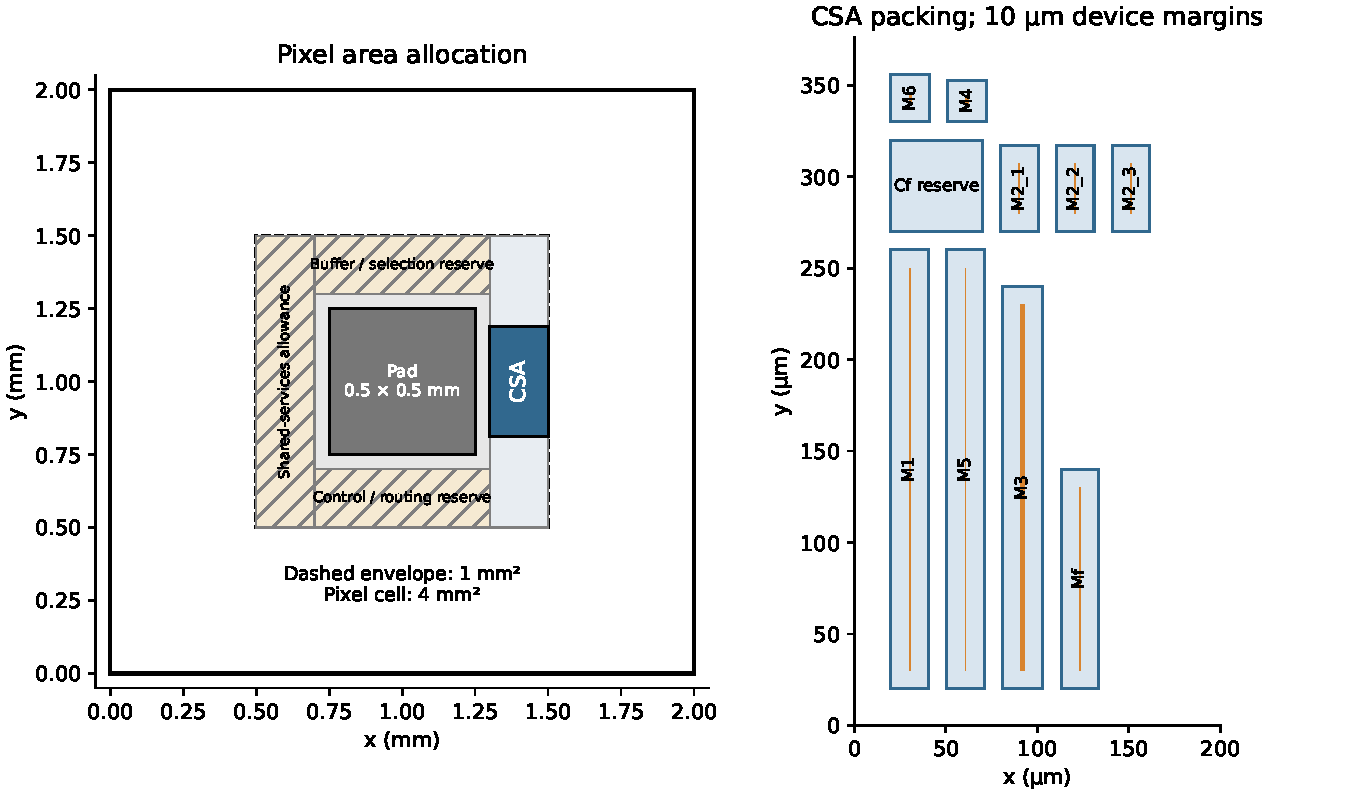
\includegraphics[width=\linewidth]{pixel_area.pdf}
\caption{Izquierda: presupuesto de 1 mm$^2$ dentro de una celda de pitch 2 mm.
Las regiones rayadas representan reservas de diseño. La región de servicios
compartidos representa su asignación por píxel. Derecha: colocación geométrica
de los canales y sus envolventes con márgenes de 10 $\mu$m.}
\end{figure}

\section*{Comparación con Topmetal-S y servicios compartidos}
Yang et al. publican un chip completo de 2,632 por 1,794 mm, es decir,
4.72181 mm$^2$. Incluye electrodo, CSA, buffer, DAC de polarización, control y
51 pads de conexión. Liang et al. publican 2,6 por 1,5 mm, 3.9 mm$^2$,
con ADC externo. Son referencias de chip completo.

Como prueba del presupuesto compartido, se toma una matriz ilustrativa de
64 píxeles y un área común igual al chip completo de Yang. Su coste
amortizado es 0.0737782 mm$^2$ por píxel, frente a la reserva de 0.2
mm$^2$. Esta comparación fija una escala de área; el circuito común de NAUSICA
se dimensionará según su propia lectura.

La matriz ilustrativa mide 16 por 16 mm. Su reserva compartida total,
12.8 mm$^2$, cabe geométricamente en dos bandas exteriores de 0.4
mm de ancho, dentro de los márgenes de 0.5 mm que quedan junto a los
envolventes centrales. Esta comprobación mantiene las posiciones de los pads
en la retícula de 2 mm. El borde de dado, protección ESD y encapsulado se
concretarán en el diseño de la matriz.

\section*{Reproducción y comprobaciones}
\texttt{config/pixel\_area.toml} contiene las hipótesis y fuentes;
\texttt{src/ion\_signal/pixel\_area.jl} calcula áreas y posiciones y guarda
HDF5. Python genera la figura y este informe a partir de ese archivo.
Se verifican la multiplicidad de M2, las dimensiones efectivas de M5, la suma
de áreas, los límites de cada región, la ausencia de solapamientos y la ley
de escala: duplicar todas las longitudes cuadruplica las áreas.
El README de resultados contiene los comandos completos.

\begin{thebibliography}{9}
\bibitem{yang} Y. Yang et al., JINST 19 (2024) C03031,
\url{https://doi.org/10.1088/1748-0221/19/03/C03031}.
\bibitem{liang} T. Liang et al., JINST 19 (2024) C04004,
\url{https://doi.org/10.1088/1748-0221/19/04/C04004}.
\bibitem{contact} GlobalFoundries, GF180MCU PDK, Contact rules,
\url{https://gf180mcu-pdk.readthedocs.io/en/latest/physical_verification/design_manual/drm_07_13.html}.
\bibitem{well} GlobalFoundries, GF180MCU PDK, Nwell rules,
\url{https://gf180mcu-pdk.readthedocs.io/en/latest/physical_verification/design_manual/drm_07_05.html}.
\end{thebibliography}
\end{document}
